\section{Contributions}


\subsection{Locality based overlay}

\begin{itemize}
	
	\item clustering
	
	\item Vivaldi + spirale

\end{itemize}

\subsection{Library for locality based algorithm}

%   * Construire des algos distribues fonctionnant en reseau est dur: couts 
% 	  impliques par la tolerance aux pannes et synchro.
%   * Ces couts sont parfois dus aux modeles de programmation.
Building distributed algorithm that works at large scale is complex: fault
tolerance, synchronization and network overhead has a cost that can have a
significant impact on performance. This cost can be the result of a bad software
architecture, or the consequence of inapropriate programming model like sharing
states between different processes (race condition).

%   * La collaboration entre processus peut se faire de deux maniere:
%       A) partage d'etat.
%       B) echange de message.
As illustrated in the last case, collaboration between ressource can be achieved
by sharing information between processes. This can be made in two ways:

\begin{description}

	\item [Shared state] : A ressource is shared between processes: it
	requires that each process waits for its turn before every use. This 
	property can be guaranteed by using locks to control acces to shared 
	ressource : processes have to wait that the ressource becomes free before
	using it.

	\item [Message passing] : Each process has its own state and collaborate
	with other processes by exchange of messages. In the case of the actor model 
	\cite{Hewitt1973}, a process becomes an \emph{actor} wich processes one
	message at a time. This is a lock free approach with no	shared state.

\end{description}

%   * les verrous sont des nids a deadlocks, c'est pourquoi on utilise le modele
%     d'acteurs dans la nouvelle version de DVMS.
Locking ressources often leads to deadlock \cite{agha:1986}, which can have
a significant impact on performance and scalability. That is why we decided to
leverage the actor model to reoarganize DVMS.

We created a new library whose role is to ease the development of distributed
application: it is based on modern piece of software (Scala and akka) based on
the actor model. This library makes intensive use of functionnal programming 
and the concept of \emph{peer actor} which hide fault tolerance and network
concerns.

\subsubsection{Peer actor abstraction}

\emph{Peer actor} is an actor that provides several features: fault tolerance,
network abstraction, communication between services. It provides an API that 
enables the fast developement of distributed application : connection between
instances of the application is automatically maintained, all efforts are 
concentrated on designing algorithms.

Peer actor contains two sub actors: \emph{notification actor} and \emph{network
overlay actor}. Notification actor enables services to subscribe to events that
will be triggered by other services. Network overlay actor is in charge of 
sending/receiving message through network. There exist two implementations of 
this network overlay actor: one is based on a chord ring, while the other is 
based on vivaldi algorithm to leverage locality properties.

\begin{figure}[h!]
  \centering
  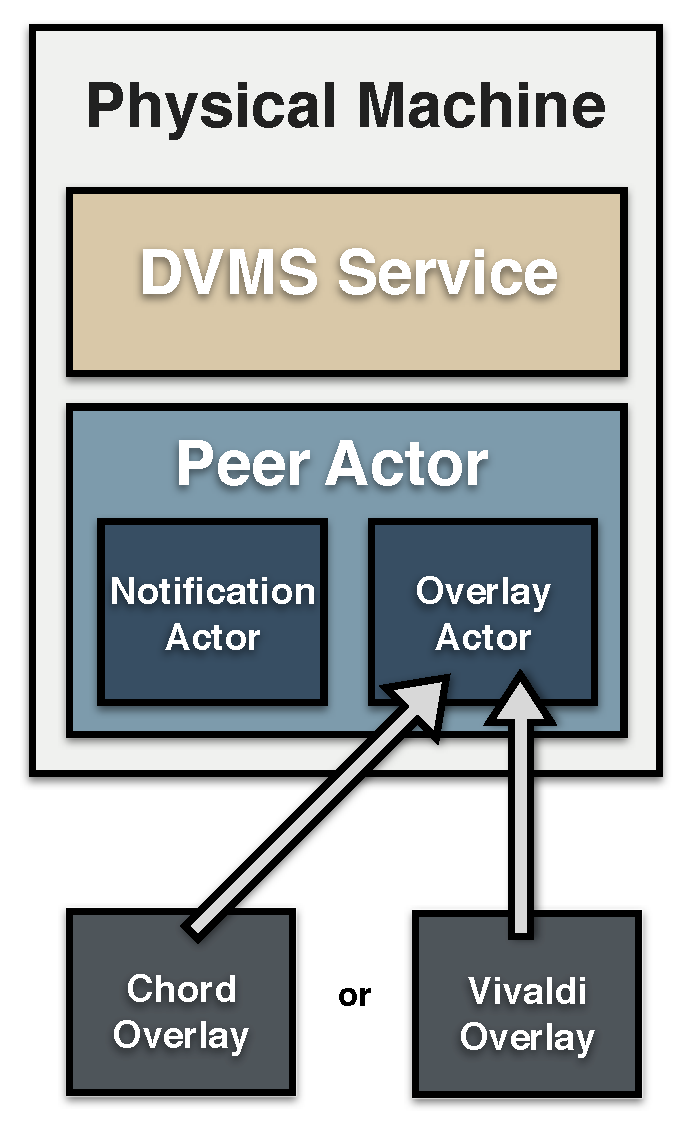
\includegraphics[width=0.5\linewidth]{Figures/DVMS.pdf}
  \caption{Architecture of DVMS based on peer actor.}%
  \label{fig:isp}%
\end{figure}

